\section{Introducción}

En el siglo~III~a.C., Eratóstenes de Cirene (c.~276--194~a.C.) midió la
circunferencia de la Tierra con una elegancia que aún sorprende.
Sabía que en el solsticio de verano el Sol iluminaba el fondo de un pozo
en Siena (hoy Asuán), indicando que el Sol estaba en el cenit, mientras
que en Alejandría proyectaba sombra.
Midiendo el ángulo de esa sombra y conociendo la distancia entre ambas
ciudades, estimó la circunferencia terrestre con notable precisión
\citep{Britannica2024}.

Nosotros reproducimos ese experimento con un \textbf{gnomon} (vara
vertical) en la plazoleta central de la Universidad de Antioquia,
Medellín, Colombia.
Realizamos dos sesiones de medición: el \textbf{19~de~marzo de~2026}
(un día antes del equinoccio vernal) y el \textbf{20~de~marzo de~2026}
(equinoccio vernal), fecha especial en la que la declinación solar es
cero y la distancia cenital al mediodía solar es exactamente igual a la
latitud geográfica del observador \citep{PortillaBarbosa2009}.
Las coordenadas del lugar de medición fueron obtenidas con Google Maps:
$(6{,}2666^\circ\text{N},\; 75{,}5694^\circ\text{O})$ \citep{GoogleMaps2026}.

% ══════════════════════════════════════════════════════════════════════════
\section{Objetivos}

\subsection{Objetivo general}

Medir experimentalmente el radio de la Tierra reproduciendo el método de
Eratóstenes, a partir de la sombra mínima proyectada por un gnomon
durante el mediodía solar y de la distancia meridional
ecuador--Medellín.

\subsection{Objetivos específicos}

\begin{itemize}
  \item Registrar la longitud de la sombra de un gnomon alrededor del
        mediodía solar en dos días consecutivos: el día anterior al
        equinoccio vernal y el propio equinoccio.
  \item Ajustar una parábola a los datos de sombra--tiempo para interpolar
        la sombra mínima y el instante del mediodía solar.
  \item Calcular la distancia cenital al mediodía solar y, a partir de
        ella, la latitud geográfica del lugar de observación.
  \item Calcular la distancia meridional entre el ecuador y Medellín
        usando el elipsoide de referencia WGS84 \citep{NGA2014}.
  \item Determinar el radio terrestre con su incertidumbre aplicando la
        propagación de errores de \citet{Baird1991}.
  \item Comparar los resultados obtenidos con el valor de referencia de
        la IAU y evaluar la concordancia estadística.
\end{itemize}

% ══════════════════════════════════════════════════════════════════════════
\section{Marco teórico}

\subsection{Geometría del gnomon}

Un \textbf{gnomon} es una vara vertical de longitud conocida $L$.
La longitud $s$ de su sombra sobre el plano horizontal depende de la
posición aparente del Sol.
Las relaciones trigonométricas relevantes son
\citep{PortillaBarbosa2009}:

\begin{equation}
  h = \arctan\!\left(\frac{L}{s}\right), \qquad
  z = 90^\circ - h = \arctan\!\left(\frac{s}{L}\right),
  \label{eq:angulos}
\end{equation}

donde $h$ es el ángulo de elevación solar y $z$ es la distancia
cenital.
La sombra es \emph{mínima} cuando el Sol cruza el meridiano del
observador, es decir, en el \textbf{mediodía solar}.

\subsection{Equinoccio y latitud geográfica}

En el equinoccio, la declinación solar es $\delta = 0^\circ$, y la altura
al mediodía en latitud $\varphi$ es \citep{PortillaBarbosa2009}:

\begin{equation}
  h_\text{mediodía} = 90^\circ - \varphi + \delta = 90^\circ - \varphi.
\end{equation}

Por lo tanto, en el equinoccio la distancia cenital al mediodía solar
es exactamente la latitud geográfica del observador:

\begin{equation}
  \boxed{z_\text{equinoccio} = \varphi}.
  \label{eq:equinoccio}
\end{equation}

Fuera del equinoccio, si $\delta \neq 0$:

\begin{equation}
  z = \varphi - \delta \quad \Rightarrow \quad \varphi = z + \delta.
  \label{eq:latitud}
\end{equation}

La declinación solar en una fecha con número de día $d$ se aproxima
mediante \citep{PortillaBarbosa2009}:

\begin{equation}
  \delta \approx 23{,}45^\circ\,\sin\!\left[\frac{360^\circ}{365}(d - 81)\right].
  \label{eq:declinacion}
\end{equation}

\subsection{Método de Eratóstenes}

Tomando el ecuador como segundo punto de referencia ($z_\text{ecuador} = 0^\circ$),
la diferencia angular es $\Delta z = \varphi$.
Si $d$ es la distancia meridional entre el ecuador y el lugar de
observación, entonces \citep{PortillaBarbosa2009,Britannica2024}:

\begin{equation}
  C = \frac{360^\circ}{\varphi} \cdot d \qquad \Longrightarrow \qquad
  \boxed{R = \frac{d}{\varphi_\text{rad}}}.
  \label{eq:radio}
\end{equation}

\subsection{Distancia meridional (WGS84)}

La distancia sobre el elipsoide WGS84 desde el ecuador hasta la
latitud $\varphi$ se calcula con la serie de Helmert
\citep{Torge2001,NGA2014}:

\begin{equation}
  M(0,\varphi) = \frac{a}{1+n}
  \Bigl[A_0\,\varphi - A_2\sin 2\varphi
        + A_4\sin 4\varphi - \cdots\Bigr],
  \label{eq:helmert}
\end{equation}

donde $a = 6\,378\,137{,}0$~m es el semieje mayor, $n = (a-b)/(a+b)$
y los coeficientes $A_i$ dependen de $n$.

\subsection{Propagación de incertidumbres}

Aplicando diferenciación total sobre $z = \arctan(s/L)$,
según \citet{Baird1991} (secciones~2-7 y~2-9):

\begin{equation}
  \delta z_\text{rad}
  = \frac{L\,\delta s + s\,\delta L}{L^2 + s^2},
  \label{eq:delta_z}
\end{equation}

y para el radio terrestre, usando la regla del producto/cociente:

\begin{equation}
  \frac{\delta R}{R} = \frac{\delta d}{d} + \frac{\delta z}{z}.
  \label{eq:delta_R}
\end{equation}

% ══════════════════════════════════════════════════════════════════════════
\section{Metodología}

\subsection{Lugar y fechas}

Las mediciones se realizaron en la plazoleta central de la
Universidad de Antioquia, Medellín, Colombia
(coordenadas: $6{,}2666^\circ\text{N}$, $75{,}5694^\circ\text{O}$,
obtenidas con Google Maps \citep{GoogleMaps2026}).
Se eligieron dos fechas: el \textbf{19~de~marzo de~2026} (un día antes
del equinoccio vernal, declinación solar $\delta_{19} \approx -1{,}21^\circ$)
y el \textbf{20~de~marzo de~2026} (equinoccio vernal,
$\delta_{20} = 0^\circ$).
La hora se registró consultando el sitio web \texttt{time.is/GMT-5}
\citep{TimeIs2026}.

\subsection{Materiales e instrumentos}

\begin{itemize}
  \item \textbf{Gnomon día 19:} vara vertical de longitud
        $L_{19} = (102{,}7 \pm 0{,}1)$~cm.
  \item \textbf{Gnomon día 20:} vara vertical de longitud
        $L_{20} = (102 \pm 0{,}1)$~cm.
  \item Plomada, para verificar la verticalidad del gnomon.
  \item Cinta métrica.
  \item Papel blanco y lápiz, para marcar el extremo de la sombra.
  \item Reloj (hora consultada en \texttt{time.is/GMT-5}).
\end{itemize}

\subsection{Procedimiento de toma de datos}

Se colocó el gnomon verticalmente sobre un plano horizontal,
usando la plomada para garantizar su perpendicularidad al horizonte
matemático. La Figura~\ref{fig:sombra_verticalidad} muestra, a la izquierda, el registro de la sombra y, a la derecha, la verificación de la verticalidad con plomada.
Se puso un papel blanco en el suelo y se marcó con un lápiz el extremo
de la sombra a intervalos irregulares, durante al menos 15~minutos antes
y 15~minutos después del mediodía solar.
Posteriormente, se midió con cinta métrica la distancia entre el pie
del gnomon y cada marca.

El intervalo entre medidas fue irregular porque en días nublados no era
posible tomar datos cada vez que una nube cubría el Sol.
El error de medición de la sombra se estimó en $\delta s_{19} = \pm 0{,}4$~cm
(día~19, gnomon grueso) y $\delta s_{20} = \pm 0{,}3$~cm (día~20).

Los datos registrados se presentan en la Tabla~\ref{tab:datos19}
(día~19) y la Tabla~\ref{tab:datos20} (día~20).

\begin{table}[H]
  \centering
  \caption{Datos de sombra del gnomon, 19~de~marzo de~2026.
           Gnomon: $L_{19} = (102{,}7 \pm 0{,}1)$~cm,
           $\delta s = \pm 0{,}4$~cm.}
  \label{tab:datos19}
  \begin{tabular}{cc}
    \toprule
    Hora (UTC$-$5) & Longitud de sombra $s$ (cm) \\
    \midrule
    11:56:30 & 14{,}8 \\
    11:58:40 & 16{,}0 \\
    12:00:00 & 15{,}0 \\
    12:07:27 & 16{,}9 \\
    12:09:29 & 16{,}3 \\
    12:12:12 & 13{,}7 \\
    12:14:40 & 15{,}4 \\
    \bottomrule
  \end{tabular}
\end{table}

\begin{table}[H]
  \centering
  \caption{Datos de sombra del gnomon, 20~de~marzo de~2026 (equinoccio).
           Gnomon: $L_{20} = (102 \pm 0{,}1)$~cm,
           $\delta s = \pm 0{,}3$~cm.}
  \label{tab:datos20}
  \begin{tabular}{cc}
    \toprule
    Hora (UTC$-$5) & Longitud de sombra $s$ (cm) \\
    \midrule
    11:57:23 & 13{,}0 \\
    12:10:51 & 11{,}3 \\
    12:12:08 & 11{,}2 \\
    12:14:37 & 11{,}3 \\
    \bottomrule
  \end{tabular}
\end{table}

\begin{figure}[H]
  \centering
  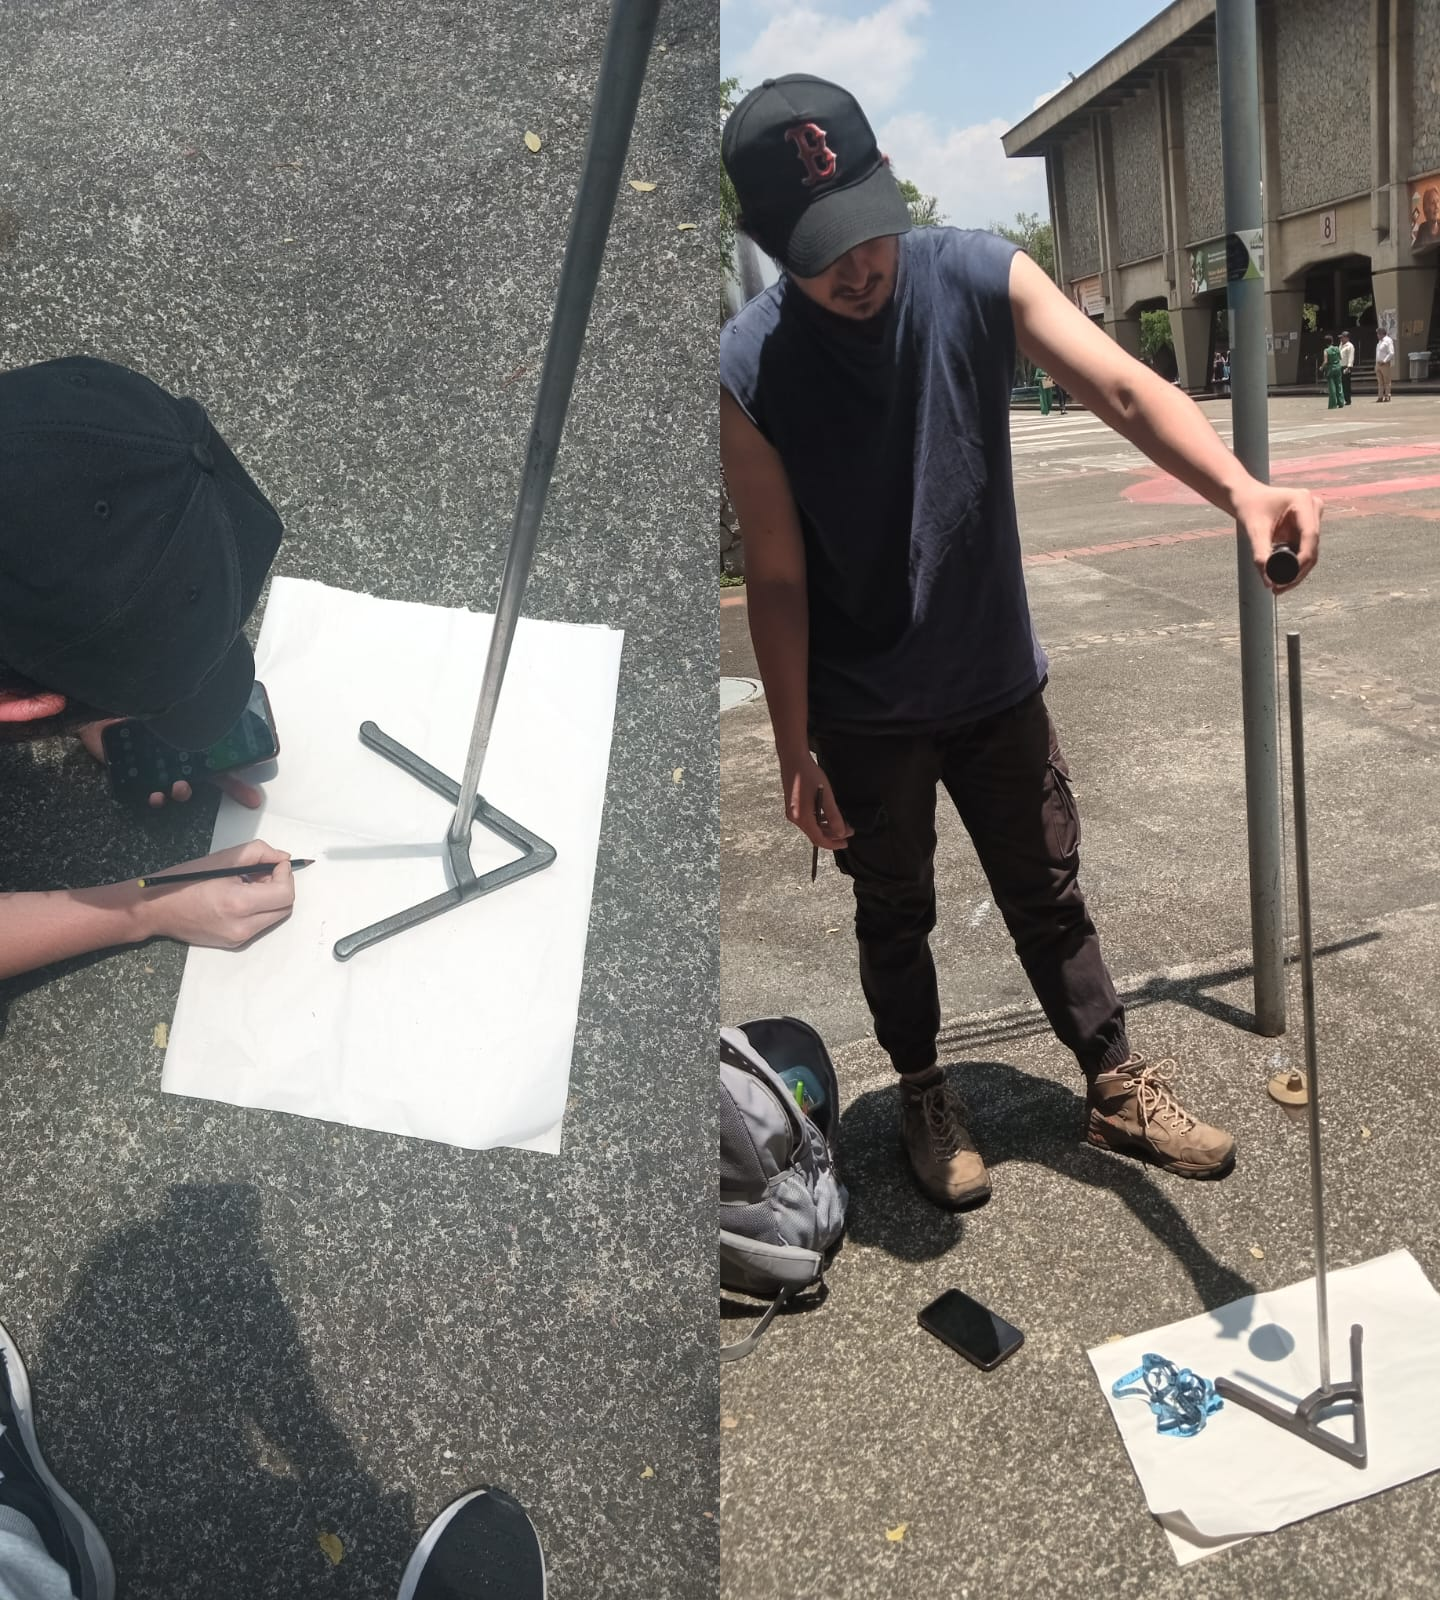
\includegraphics[width=0.68\textwidth]{imagenes/Sombra-Verticalidad.png}
  \caption{Registro experimental durante la toma de datos: a la izquierda se observa la medición de la longitud de la sombra y a la derecha la verificación de la verticalidad del gnomon con plomada.}
  \label{fig:sombra_verticalidad}
\end{figure}

% ══════════════════════════════════════════════════════════════════════════
\section{Análisis de datos y resultados}

\subsection{Ajuste parabólico}

La longitud de la sombra varía de forma casi cuadrática con el tiempo
alrededor del mediodía solar.
Se ajustó el modelo $s(t) = a\,(t - t_0)^2 + s_\text{min}$ por
mínimos cuadrados a cada conjunto de datos (Figura~\ref{fig:sombra_tiempo}).
Los parámetros de interés son $s_\text{min}$ (sombra mínima ajustada)
y $t_0$ (estimado del mediodía solar).

\begin{figure}[H]
  \centering
  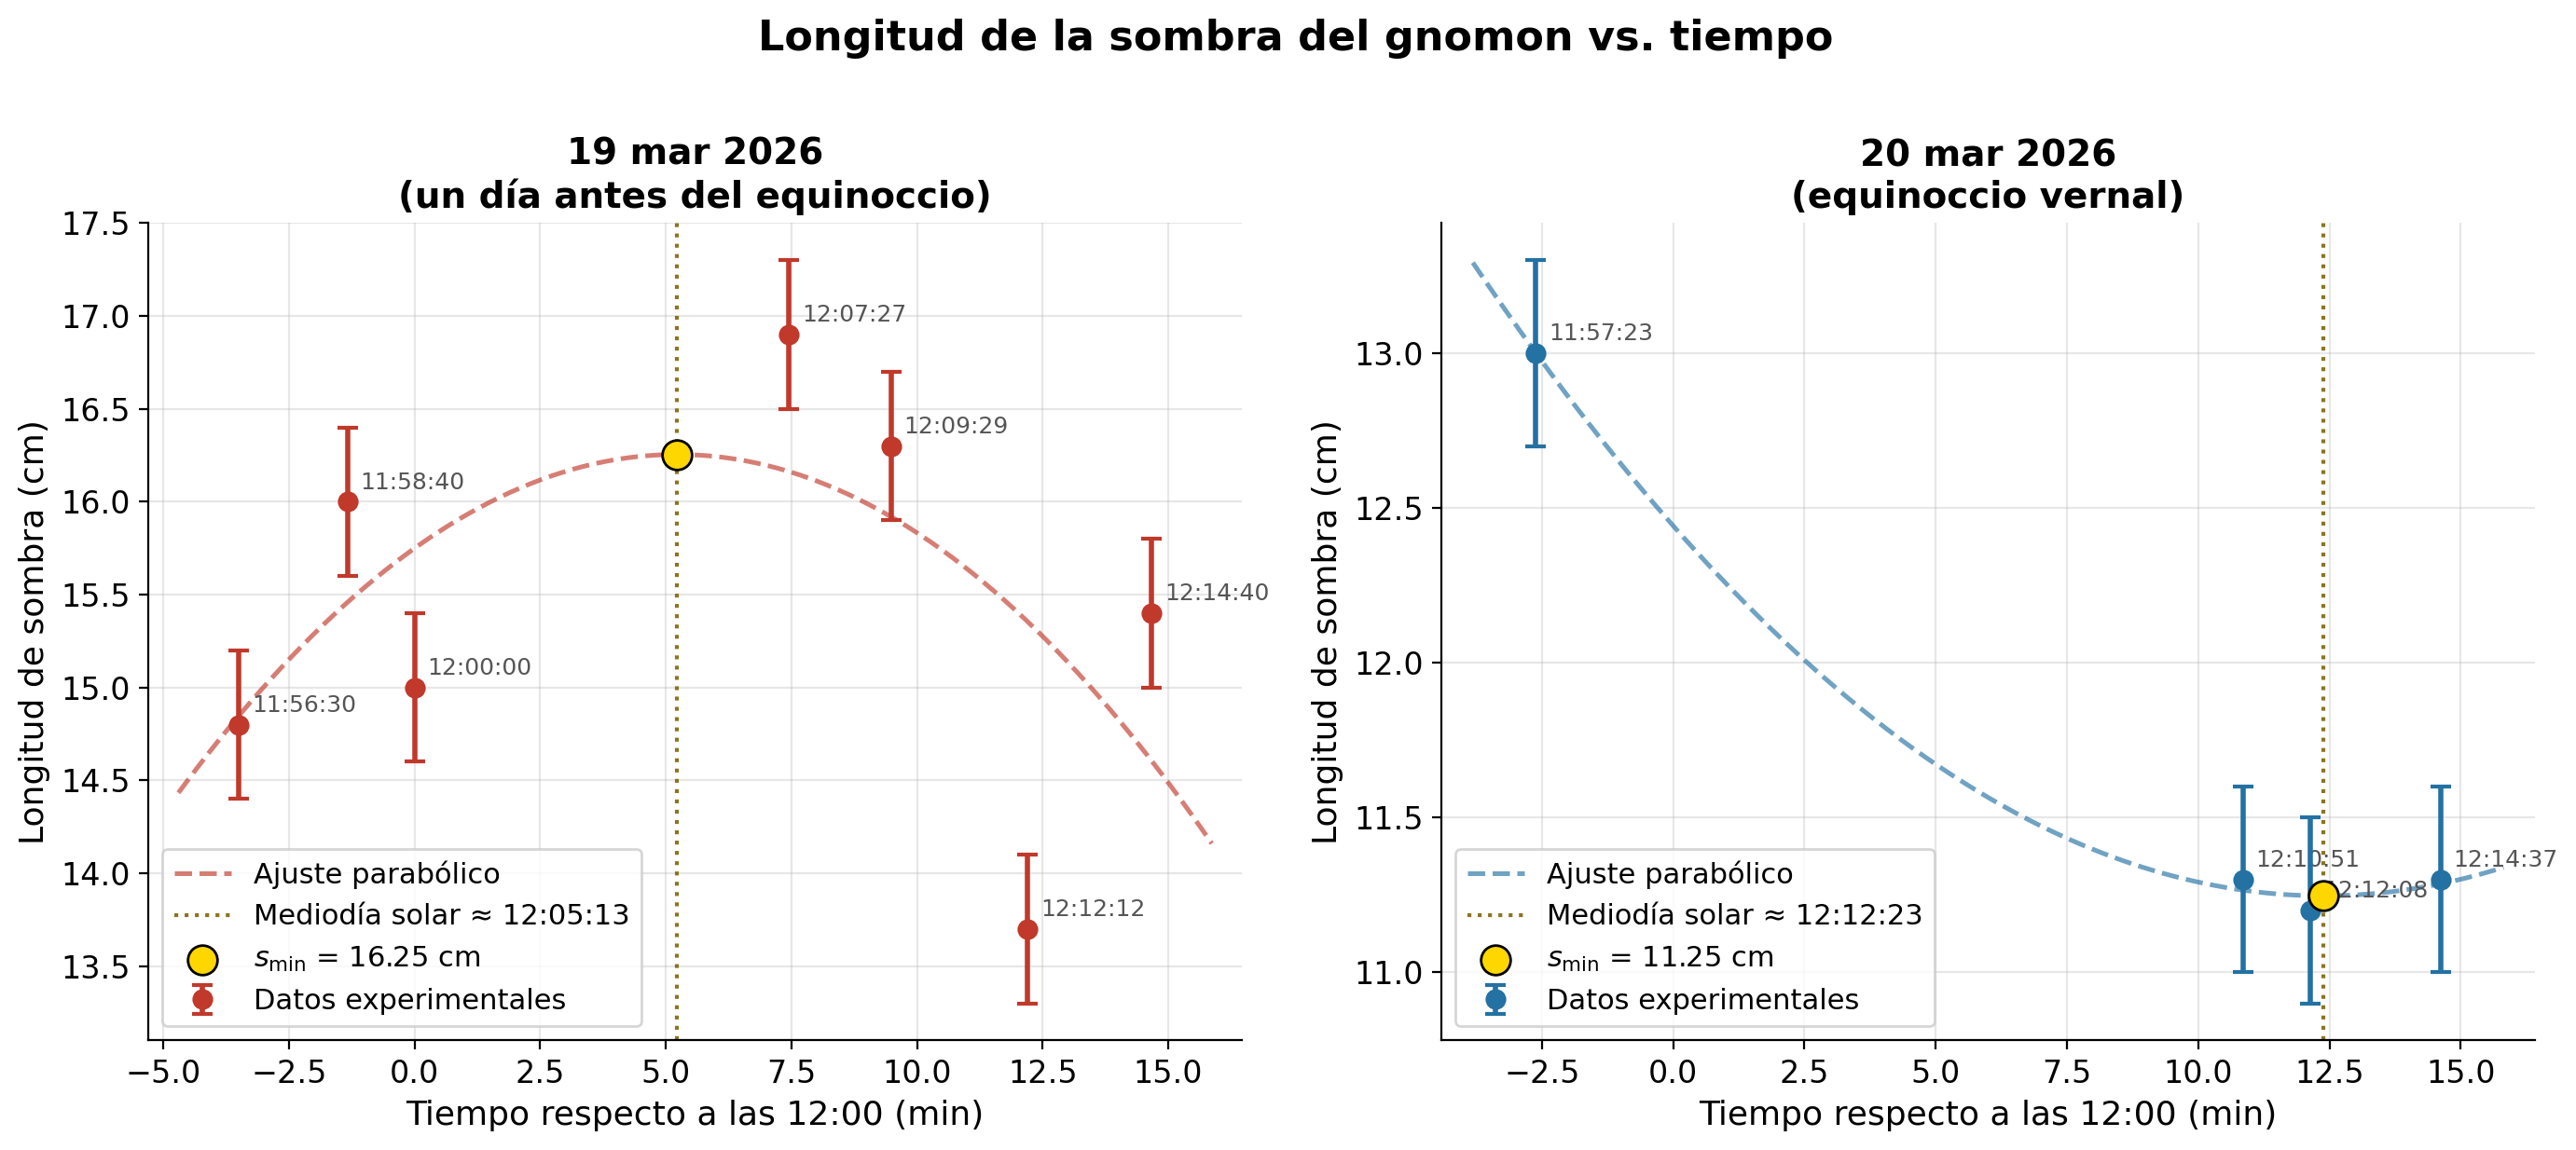
\includegraphics[width=\textwidth]{imagenes/fig1_sombra_vs_tiempo.png}
  \caption[Longitud de sombra del gnomon en función del tiempo]{Longitud de sombra del gnomon en función del tiempo para el
           19 y el 20~de~marzo de~2026.
           Las curvas corresponden al ajuste parabólico
           $s(t) = a(t-t_0)^2 + s_\text{min}$.
           Las barras de error horizontales y verticales representan la
           incertidumbre en la hora ($\pm 1$~s) y en la longitud de la
           sombra, respectivamente.}
  \label{fig:sombra_tiempo}
\end{figure}

\textbf{Día 20 (equinoccio):} El ajuste es satisfactorio con 4~puntos.
La sombra mínima ajustada ($s_{\min,20}^\text{fit} \approx 11{,}25$~cm)
coincide con el mínimo observado ($11{,}2$~cm) dentro de la
incertidumbre de medición.
Se usa el valor ajustado para los cálculos.

\textbf{Día 19:} El ajuste parabólico \emph{falla} porque los datos no
siguen un patrón parabólico limpio.
El mínimo ajustado ($\approx 16{,}26$~cm) es mayor que el mínimo
observado ($13{,}7$~cm), lo que se atribuye a la falta de soporte rígido
del gnomon y a la distribución asimétrica de los datos alrededor del
mínimo.
Para el día~19 se usa el \textbf{mínimo observado directamente}
($s_{19} = 13{,}7$~cm); el parámetro~$t_0$ del ajuste sí es útil
para estimar el instante del mediodía solar.

\subsection{Diagrama geométrico del gnomon}

La Figura~\ref{fig:gnomon} ilustra la geometría del experimento:
el gnomon vertical de longitud $L$, la sombra de longitud $s$ y los
ángulos $h$ (elevación solar) y $z$ (distancia cenital).

\begin{figure}[H]
  \centering
  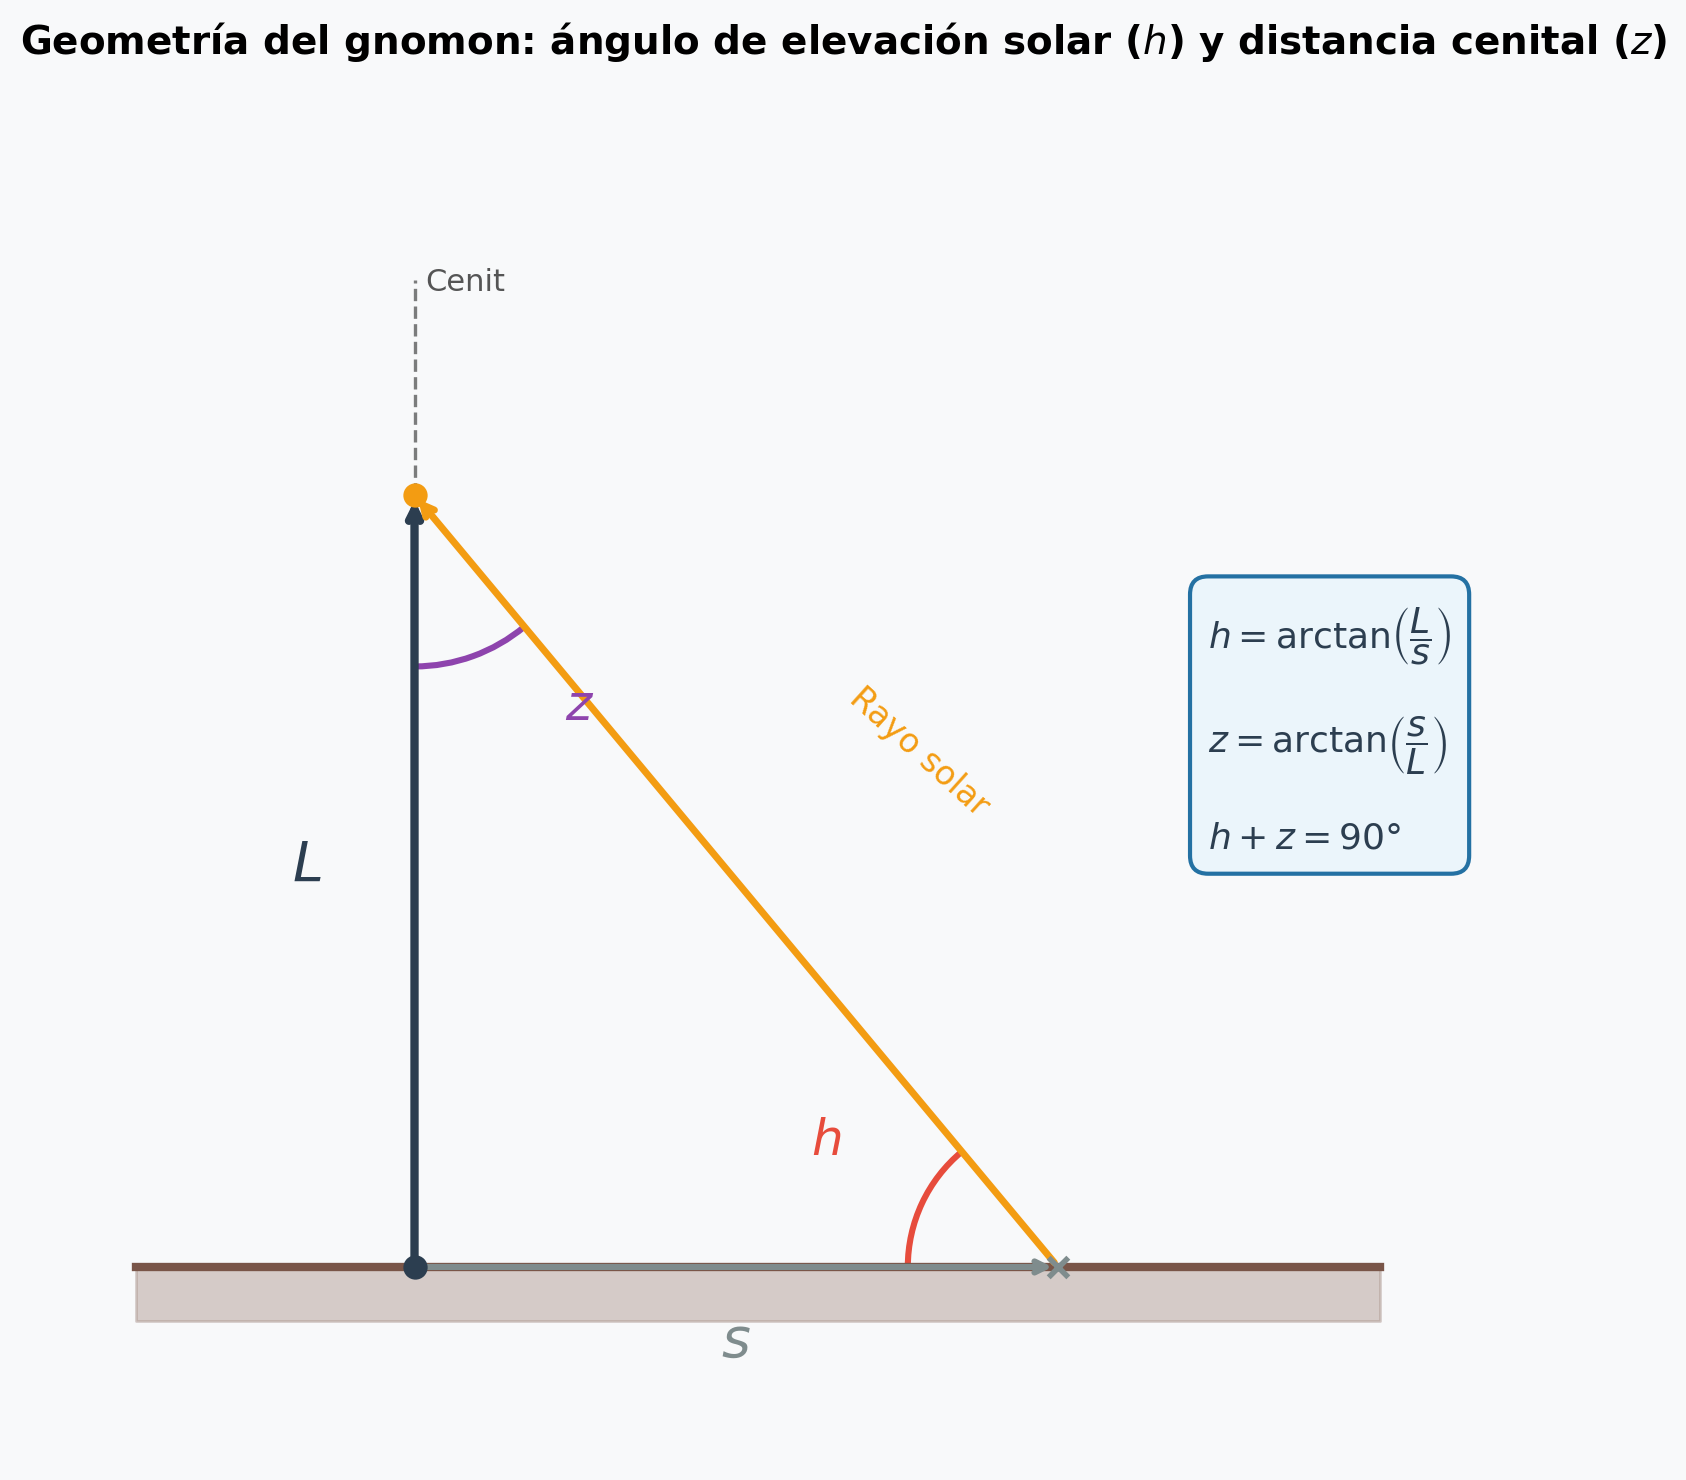
\includegraphics[width=0.7\textwidth]{imagenes/fig2_diagrama_gnomon.png}
  \caption{Diagrama geométrico del gnomon.
           El ángulo de elevación solar $h$ y la distancia cenital
           $z = 90^\circ - h$ se obtienen a partir de las longitudes $L$
           (gnomon) y $s$ (sombra) mediante las
           ecuaciones~(\ref{eq:angulos}).}
  \label{fig:gnomon}
\end{figure}

\subsection{Distancia cenital y latitud}

Con la sombra mínima seleccionada para cada día, se aplica la
ecuación~(\ref{eq:angulos}) para obtener la distancia cenital~$z$.
En el equinoccio ($\delta_{20} = 0^\circ$), la ecuación~(\ref{eq:equinoccio})
da directamente la latitud: $\varphi = z_{20}$.
Para el día~19 se aplica la corrección~(\ref{eq:latitud})
con la declinación calculada mediante la ecuación~(\ref{eq:declinacion}):
$\delta_{19} \approx -1{,}21^\circ$.

La Figura~\ref{fig:latitud} compara las latitudes calculadas con la
latitud real del lugar.

\begin{figure}[H]
  \centering
  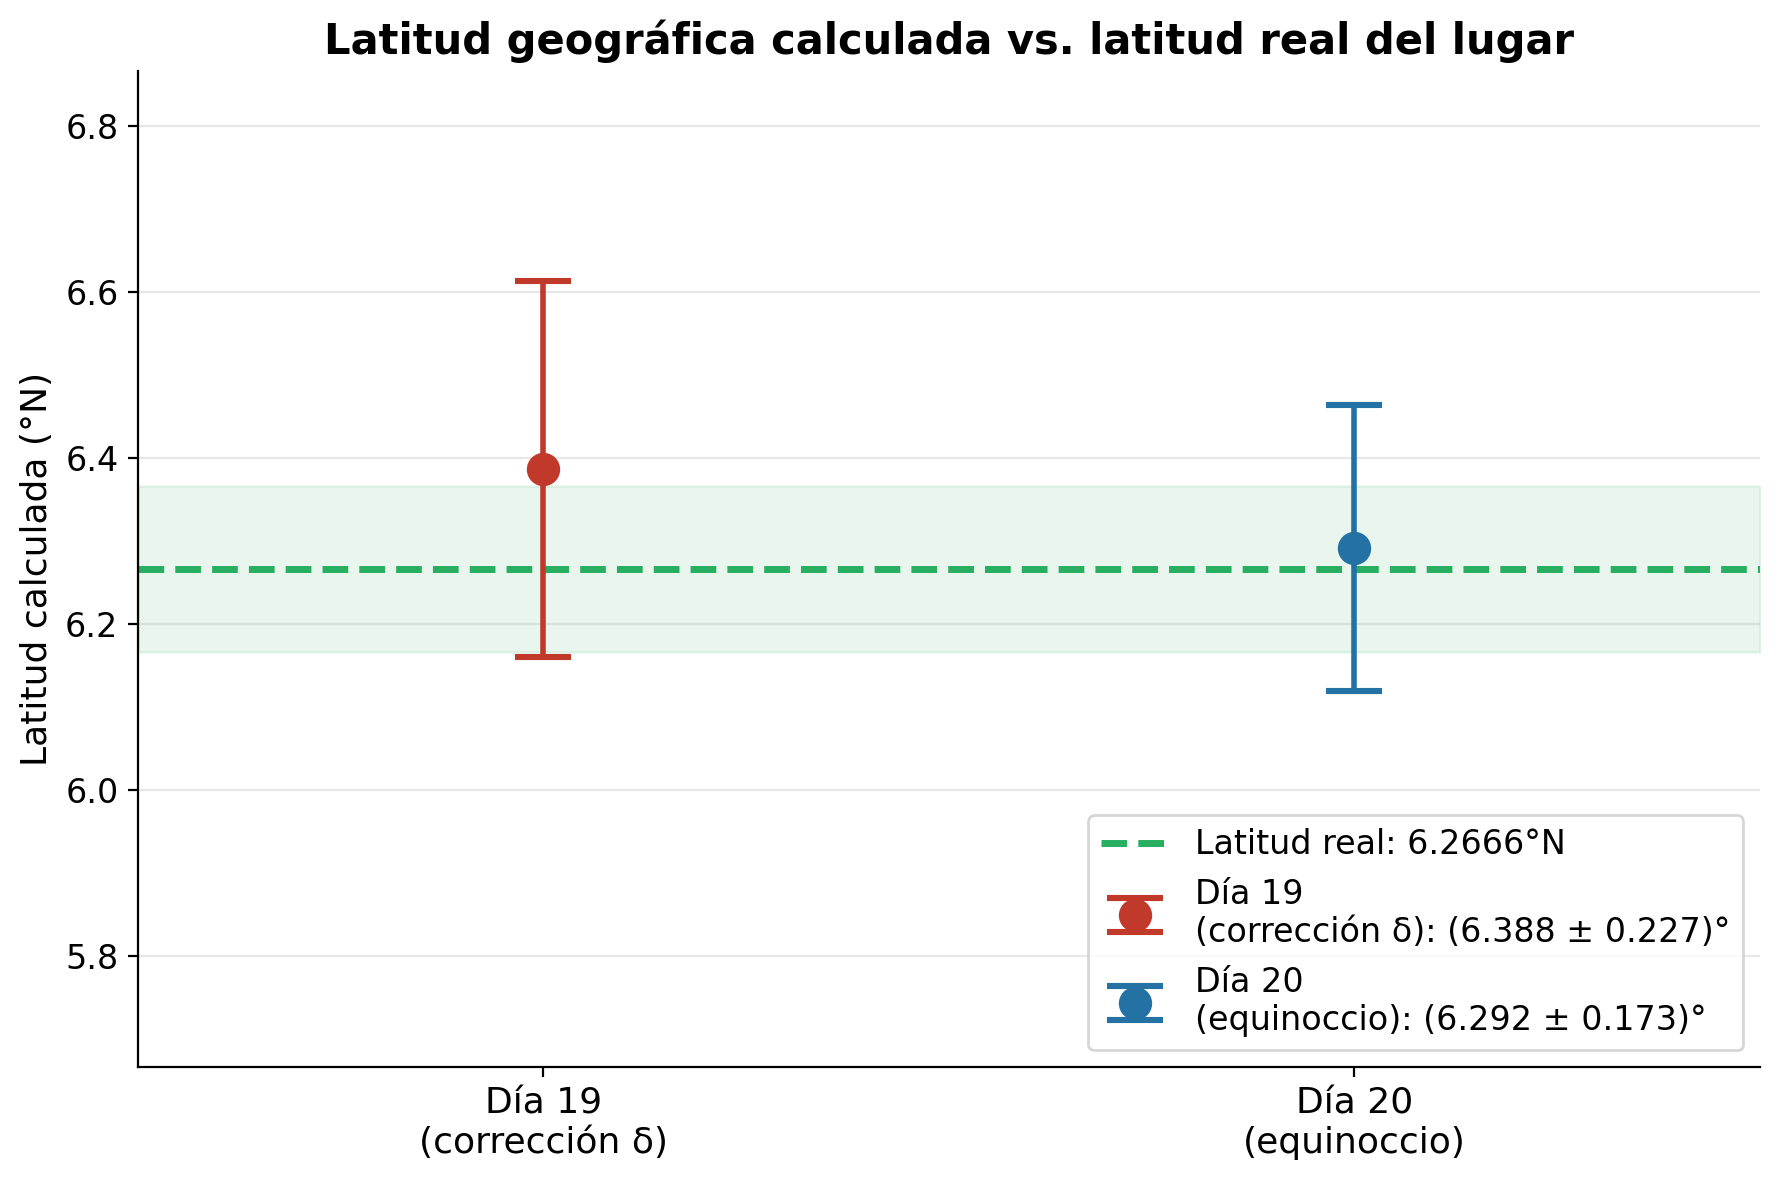
\includegraphics[width=0.8\textwidth]{imagenes/fig4_latitud_calculada.png}
  \caption{Comparación de la latitud calculada (con su incertidumbre)
           y la latitud real del lugar de observación
           ($\varphi_\text{real} = 6{,}2666^\circ$N).}
  \label{fig:latitud}
\end{figure}

\subsection{Distancia meridional}

La distancia meridional desde el ecuador hasta la latitud del
observador se calculó usando la serie de Helmert sobre el elipsoide
WGS84 \citep{Torge2001,NGA2014}, ecuación~(\ref{eq:helmert}):

\[
  d = (695{,}9 \pm 1{,}0)~\text{km}.
\]

La incertidumbre de $\pm 1$~km es conservadora y tiene en cuenta la
precisión de las coordenadas GPS y el modelo geométrico.

\subsection{Radio terrestre}

Aplicando la ecuación~(\ref{eq:radio}) con la propagación de
incertidumbres~(\ref{eq:delta_R}) \citep{Baird1991},
se obtienen los resultados de la Tabla~\ref{tab:resultados}.
La Figura~\ref{fig:radio} ilustra visualmente la comparación con el
valor de referencia de la IAU.

\begin{table}[H]
  \centering
  \caption{Resumen de resultados: radio terrestre calculado comparado
           con el valor de referencia de la IAU
           ($R_\text{ref} = 6\,371$~km).}
  \label{tab:resultados}
  \begin{tabular}{lccc}
    \toprule
    Sesión & $R$ calculado (km) & Error relativo & $R_\text{ref} \in [R \pm \delta R]$? \\
    \midrule
    Día 20 --- equinoccio (principal)    & $6\,310 \pm 182$ & 0{,}96\,\% & Sí \\
    Día 19 --- corrección de $\delta$    & $6\,215 \pm 229$ & 2{,}44\,\% & Sí \\
    Media ponderada                      & $6\,273 \pm 143$ & 1{,}53\,\% & Sí \\
    \bottomrule
  \end{tabular}
\end{table}

\begin{figure}[H]
  \centering
  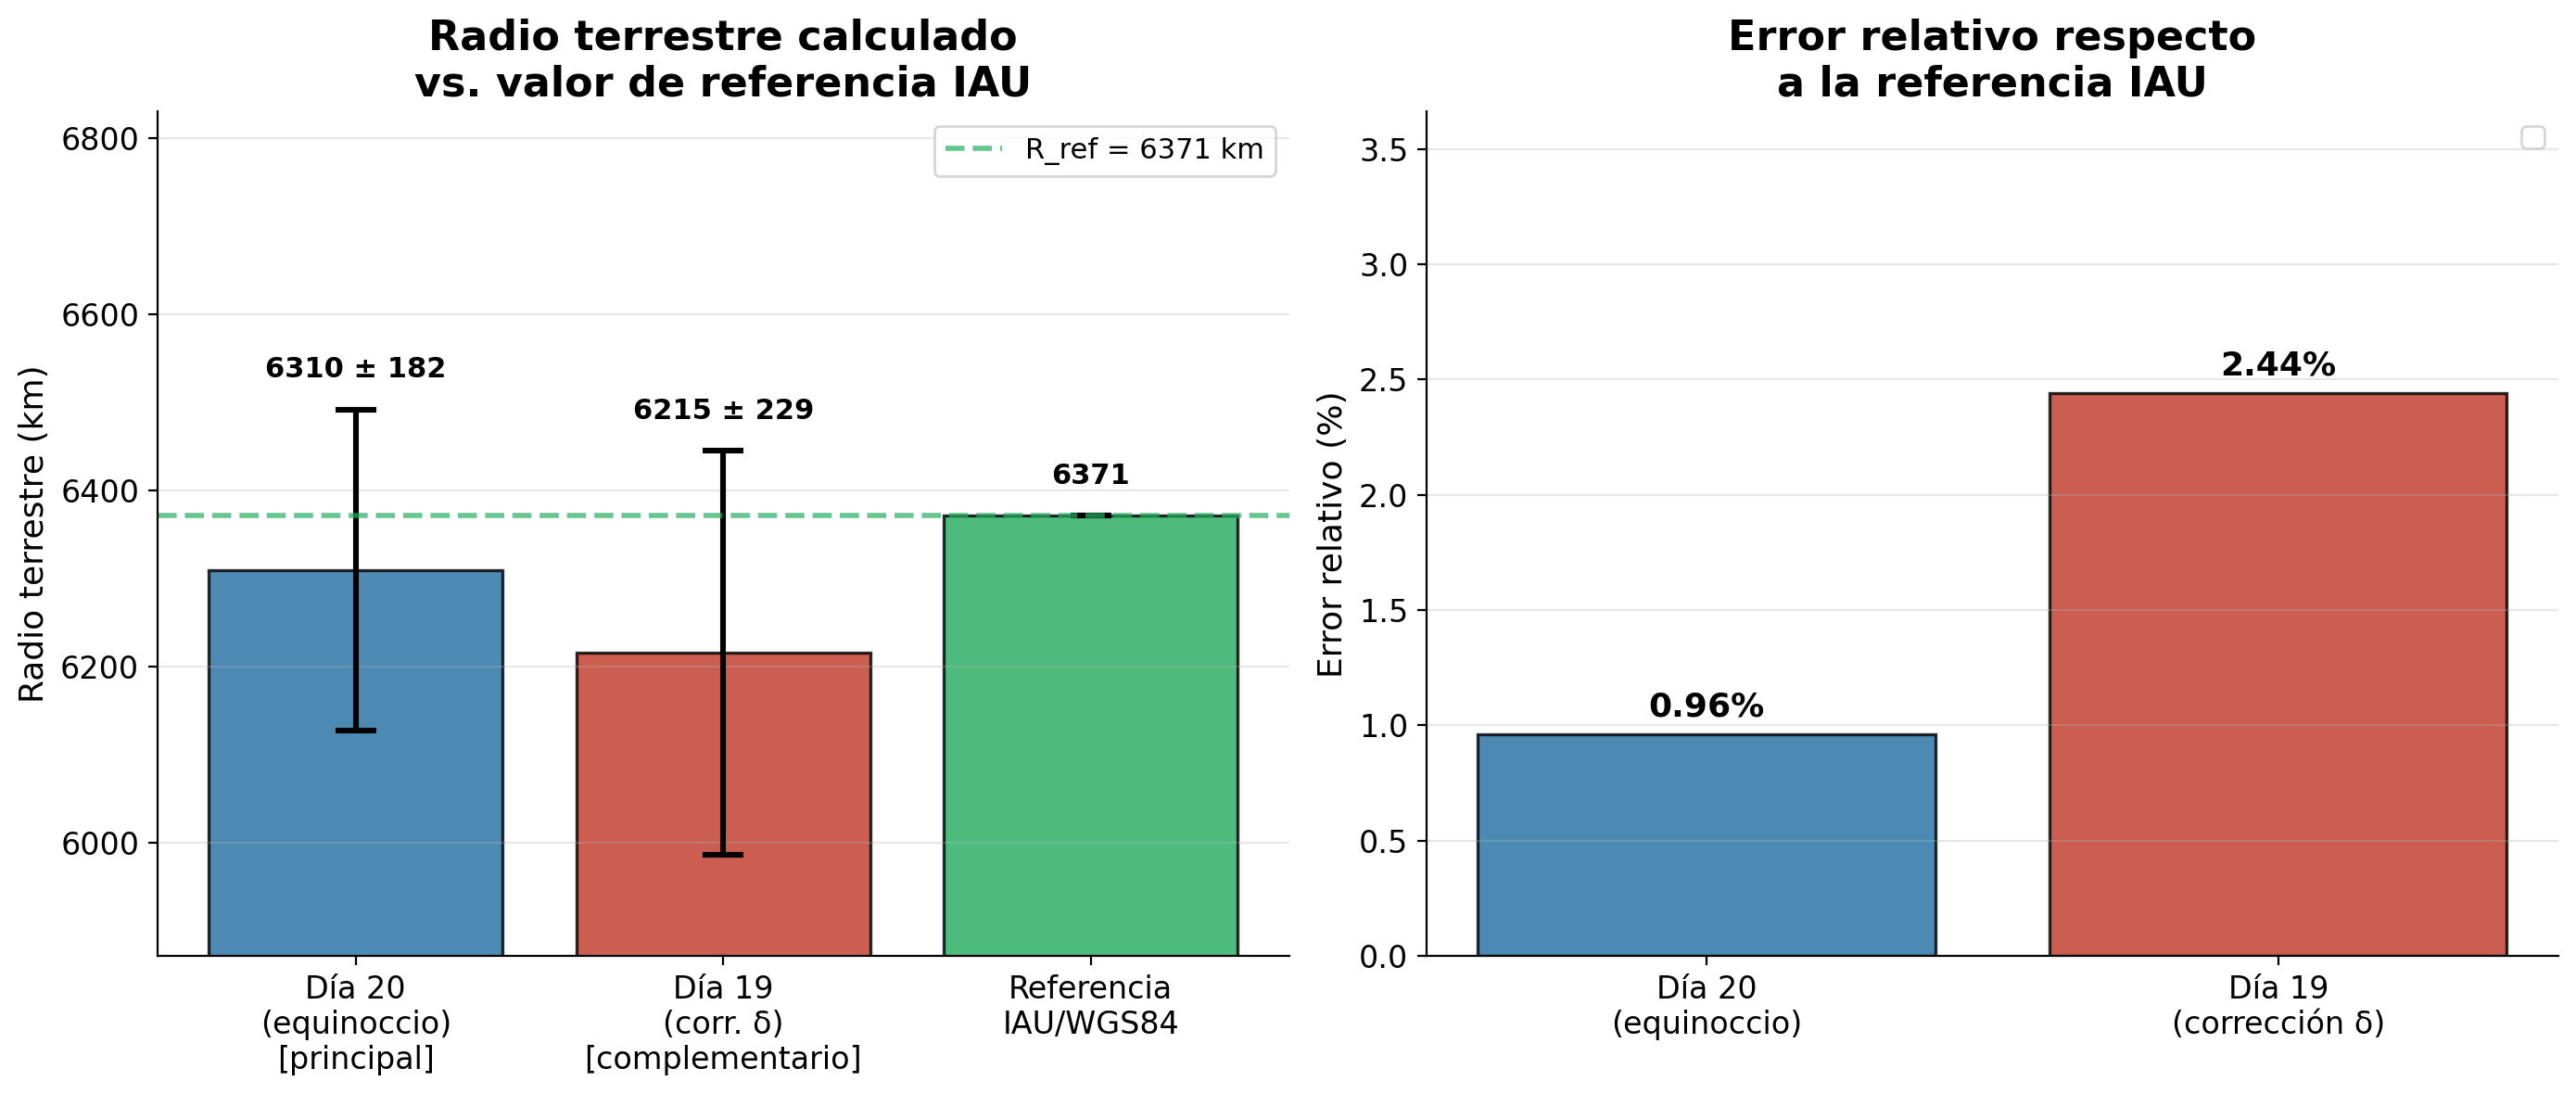
\includegraphics[width=\textwidth]{imagenes/fig3_comparacion_radio.png}
  \caption[Comparación del radio terrestre calculado]{Comparación del radio terrestre calculado con el valor de
           referencia IAU/WGS84 ($R_\text{ref} = 6\,371$~km).
           \emph{Izquierda:} barras de radio calculado con intervalos
           de incertidumbre; la línea horizontal verde indica el valor
           de referencia.
           \emph{Derecha:} error porcentual de cada resultado.}
  \label{fig:radio}
\end{figure}

% ══════════════════════════════════════════════════════════════════════════
\section{Discusión}

\subsection{Precisión de los resultados}

Ambos resultados incluyen el valor de referencia IAU ($R = 6\,371$~km)
dentro de su intervalo de incertidumbre (Tabla~\ref{tab:resultados}).
El resultado del equinoccio es el más preciso, con un error inferior
al 1\,\%.
Las barras de error de ambos días se superponen con el valor de
referencia, lo que confirma la consistencia estadística de las
mediciones.
La barra de error del día~20 es notablemente más corta que la del
día~19, reflejando la mayor precisión obtenida durante el equinoccio
gracias a las mejores condiciones del gnomon y a la geometría
simplificada ($z = \varphi$).

\subsection{Ventaja del equinoccio}

La medición del 20~de~marzo es la más directa: en el equinoccio, la
distancia cenital al mediodía solar es exactamente la latitud geográfica
\citep{PortillaBarbosa2009}, sin necesidad de corregir por la
declinación solar.
La pequeña declinación del día~19 ($\delta \approx -1{,}21^\circ$) introduce
una corrección adicional y una fuente extra de incertidumbre.

\subsection{Ajuste parabólico: éxito y limitaciones}

El ajuste parabólico fue exitoso para el día~20 (4~puntos con baja
dispersión): la sombra mínima interpolada ($\approx 11{,}25$~cm)
coincide con el mínimo observado ($11{,}2$~cm) dentro de la
incertidumbre de medición, lo que permite estimar con mayor precisión
el momento del mediodía solar.

Para el día~19, el ajuste falló porque los datos presentan alta
dispersión ocasionada por la falta de soporte rígido del gnomon, por
su mayor grosor y por la distribución asimétrica de los datos
alrededor del mínimo (no se tomaron datos en el intervalo 12:00--12:07
por condiciones de nubosidad).
Por ello, para los cálculos del día~19 se usó el mínimo observado
directamente ($13{,}7$~cm).
Esta distinción ilustra la importancia de evaluar la calidad de los
ajustes estadísticos antes de usarlos en cálculos físicos
\citep{Baird1991}.

\subsection{Mediodía solar}

Los ajustes parabólicos ubican el mediodía solar alrededor de las
12:05--12:12.
El mediodía solar teórico para la longitud $-75{,}57^\circ$ con la ecuación
del tiempo del 20~de~marzo ($\approx +7$~min) es
$t_\text{noon} \approx 12{:}09$.
La estimación del día~20 ($\approx 12{:}12$) difiere en menos de
3~minutos, lo cual es razonable dado el número reducido de datos.

\subsection{Fuentes de error}

El análisis de propagación de incertidumbres muestra que:

\begin{enumerate}
  \item \textbf{Incertidumbre en la longitud de la sombra} ($\delta s$):
        fuente dominante (70--80\,\% del error total), causada
        por el grosor del gnomon y la dificultad de marcar con precisión
        el extremo de la sombra.
  \item \textbf{Incertidumbre en la distancia meridional} ($\delta d$):
        segunda contribución (15--25\,\%).
  \item \textbf{Incertidumbre en el gnomon} ($\delta L$): contribución
        menor al 5\,\%.
\end{enumerate}

Como mejoras se proponen: usar un gnomon más delgado (alambre o lápiz)
para una sombra más nítida; emplear un soporte rígido con nivel de
burbuja; tomar medidas cada 2--3~minutos durante al menos 20~minutos
alrededor del mediodía solar; y registrar fotográficamente la posición
de la sombra para mayor precisión.

\subsection{Comparación histórica}

La estimación original de Eratóstenes ($C \approx 39\,375$~km,
$R \approx 6\,267$~km) tiene un error de 1{,}6\,\% respecto al
valor moderno \citep{Britannica2024}.
Nuestra medición principal (error 0{,}96\,\%) logra mayor
precisión con instrumentos igualmente simples, gracias al
aprovechamiento del equinoccio y al conocimiento preciso de la latitud
del lugar (coordenadas GPS).

% ══════════════════════════════════════════════════════════════════════════
\section{Conclusiones}

\begin{enumerate}
  \item Se midió experimentalmente el radio terrestre usando el método
        de Eratóstenes con datos tomados en la plazoleta de la
        Universidad de Antioquia.
        El resultado principal (equinoccio, 20~de~marzo) es
        $R_{20} = (6\,310 \pm 182)$~km, con un error relativo del
        0{,}96\,\% respecto al valor de la IAU; el valor real cae
        dentro del intervalo de incertidumbre.

  \item La condición de equinoccio simplifica el método: la distancia
        cenital al mediodía solar ($z_{20} \approx 6{,}29^\circ$) coincide
        directamente con la latitud geográfica del lugar, sin necesidad
        de corregir por la declinación solar \citep{PortillaBarbosa2009}.

  \item El ajuste parabólico fue exitoso para el día~20 y permitió
        interpolar la sombra mínima y el mediodía solar con mayor
        precisión.
        Para el día~19, el ajuste falló debido a la alta dispersión de
        los datos, obligando a usar el mínimo observado directamente.
        Esta distinción ilustra la importancia de evaluar la calidad
        de los ajustes estadísticos antes de usarlos en cálculos físicos
        \citep{Baird1991}.

  \item La latitud calculada desde el equinoccio
        ($z_{20} \approx 6{,}29^\circ$N) coincide con la latitud real
        ($6{,}2666^\circ$N) con una diferencia de apenas $0{,}026^\circ$,
        confirmando la solidez del método.

  \item La fuente de error dominante es la incertidumbre en la
        medición de la longitud de la sombra (70--80\,\% del
        error total).
        Usar un gnomon más delgado y un soporte rígido con nivel
        reduciría significativamente el error.

  \item Este experimento demuestra que, con materiales básicos, un
        gnomon y conocimientos elementales de geometría y trigonometría,
        es posible reproducir la hazaña de Eratóstenes con una
        precisión inferior al 1\,\%, replicando un logro científico
        de hace más de dos mil años.
\end{enumerate}

% ══════════════════════════════════════════════════════════════════════════
